\documentclass[11pt]{article}
\usepackage{amsmath,amsthm,amssymb}
\usepackage{mathtools}
\usepackage{enumerate}
\usepackage{graphicx}
\usepackage{mathpazo}
\usepackage{lmodern}
\usepackage{parskip}
\usepackage{fancyhdr}
\usepackage{wrapfig}
\usepackage{tikz}
\usepackage{hyperref}
\usepackage{listings}
\usepackage[linesnumbered,algoruled,boxed,lined]{algorithm2e}
\usetikzlibrary{positioning}
\newtheorem{theorem}{Theorem}
\newtheorem{defn}{Definition}
\newcommand{\Jostle}{\texttt{Jostle}}
\lhead{Senior Thesis}
\rhead{Jacob Imola}
\cfoot{\thepage}
\pagestyle{fancy}
\title{Automatic, Fine-Grained Algorithmic Choice for DP}
\date{\today}
\author{Jacob Imola\\ School of Computer Science, Carnegie Mellon University\and Jean Yang\\ School of Computer Science, Carnegie Mellon University}
\begin{document}
\maketitle
\section{Introduction}
The rapid technological increase in data collection, speed, and storage has brought about revolutionary insights and ideas and will continue to do so. However, with huge amounts of private data comes the concern of preventing data from ending up in the wrong hands. In order to prevent data leakage, we must lay a strong privacy foundation and give data analysts the tools for them to implement privacy efficiently and correctly.

Consider a healthcare database with records like patient weight, age, some genetic information, or whether they are HIV positive. Granting access rights, or policies, to just patients and their doctors protects as much privacy as possible, and developing tools for verifying information flow policies is an interesting question in its own right. However, sometimes it's okay to release a few general statistics about a database so that an analyst can find risk factors for people who have HIV. On the other side of the spectrum, publicly releasing the entire database doesn't protect privacy at all, yet it would be an analyst's dream. In order to appease both data analysts and patients, a middle ground area must be chosen where a blurry snapshot of the database is released, comprehensive enough so that meaningful conclusions may be drawn yet blurry enough so that individuals are mostly protected. We call this the \emph{privacy-accuracy} tradeoff. We can always sacrifice one for the other before we disclose our database snapshot. However, after we disclose, it is impossible to take any privacy back, so we have to be absolutely sure that privacy guarantee will not fail under any attack. The most promising method for doing such a disclosure is Differential Privacy \cite{Dwork:2006}.

Differential Privacy (DP) is considered to be the gold-standard of privacy and has been researched intensely since its conception in 2005. Its goal is to provide guarantees on what can be done with the information being released from a dataset making minimal assumptions about an attacker's powers. Previous attempts were not mathematically rigorous and did not reliably prevent attacks. Notably, before DP, researchers were able to reidentify users in a Netflix dataset given an auxiliary dataset from IMDB and form a generalized attack against the state-of-the-art privacy algorithms of the time \cite{Narayanan:2006}. The strong privacy guarantee of DP, on the other hand, has a rigorous mathematical foundation that makes it impervious to the post-processing attacks that exploited the Netflix dataset, and more recently, \href{https://hackernoon.com/how-to-rob-an-airbnb-252e7e7eda44}{AirBnB} and \href{https://gizmodo.com/this-is-almost-certainly-james-comey-s-twitter-account-1793843641}{Instagram}. Differential Privacy has certainly stood the test of time as a sturdy way to protect privacy.

However, just building a suite of DP algorithms is not satisfactory. Privacy adds a new layer of complexity to the data analyst's job because the performance of algorithms may vary wildly depending on the database or on other parameters, complexity that an analyst may not fully understand. Most data analysts are not Differential Privacy experts. This leads to the central problem of this work: 

\textbf{Problem:} How can we help data analysts dispatch Differential Privacy algorithms in a way that helps them understand the privacy and accuracy tradeoff space?

This problem is noted by the authors of DPComp \cite{Hay:2016}, who comment that currently, ``the practitioner is lost and incapable of deploying the right algorithm''. DPComp allows the analyst to visualize the performances of different histogram querying algorithms on certain datasets. An example dataset  is shown in Figure \ref{fig:dpcomp}. We feel this is a step in the right direction, but there are two main drawbacks: their visualization tools are limited to 2D histogram algorithms, and they don't help the programmer enough on his actual dataset, instead using publicly available knowledge. To address both of these issues, we take a programming-language-based approach. The approach is to move the manual exploration of algorithms that an analyst might do with DPComp into the runtime of our programming language, which we call \Jostle{}. This will preserve the insights that an analyst may gleam from DPComp (since the algorithmic choice will be publicly available to him) and will confer the advantages of a programming language:

\begin{figure}
\begin{center}
\includegraphics[scale=0.3]{DPComp}
\end{center}
\caption{A screenshot of a DPComp graph depicting the original dataset and the noise that a DP algorthm, DAWA \cite{Li:2014}, adds at $\epsilon=0.01$. This would help an analyst decide whether to apply DAWA on his own dataset.}\label{fig:dpcomp}
\end{figure}
\begin{itemize}
\item \textbf{Abstraction} Creating an abstraction for algorithmic choice in a programming language allows for the suppression of complicated privacy machinery, allowing analysts to view the choice as a black box. In fact, a programmer could view all of DP as a black box and still use \Jostle{} by simply trying many DP black boxes and knowing that the best algorithm will be used \footnote{We could call these programmers privacy-agnostic.}. Programmers write code faster with fewer bugs when they can think about complicated ideas as black boxes.
\item \textbf{Generalization} As previously noted, it is infeasible to conduct experiments like DPComp on all use cases that an analyst may encounter. Writing a sophisticated programming language that automatically makes this choice would eliminate the need for this while still allowing for high-grade code performing as if the experiments had been conducted.
\end{itemize}

The most central idea in \Jostle{} is the \texttt{NoisyIf} statement, illustrated in Figure \ref{fig:1}.
\begin{figure}
\begin{lstlisting}
def f(D):
    NoisyIf(g D):
        do A
    else:
        do B
\end{lstlisting}
\caption{Example \texttt{NoisyIf} statement.}
\label{fig:1}
\end{figure}
A programmer will use \texttt{NoisyIf} when they are unsure of which choice to make at a certain point in their code. If they have certain beliefs that may aid \Jostle{} in making the choice, then they may specify an \emph{advice} function (denoted by \texttt{g} in Figure \ref{fig:1}). Jostle will combine this advice along with previous executions of this particular \texttt{NoisyIf} to make the best decision.

We will begin with a background section on DP and related work. Then we will introduce decision trees and highlight the existence of Problem with them. Thirdly, we will solve the decision tree problem with different \texttt{NoisyIf} statements, and finally, we will illustrate how \texttt{NoisyIf} statements can be generalized to make \texttt{Jostle}.

\section{Background}
\subsection{Differential Privacy}
DP is motivated by the example of a subject being asked to participate in a study involving an algorithm $\mathcal{A}$ being run on a database $D$. If $\mathcal{A}(D)$ changes as a result of the subject participating, then this poses a privacy concern. An attacker may be able to infer something about the participant's input. This means that non-trivial deterministic algorithms are already unacceptable; their output may change depending on just a single addition to $D$. The strength $\epsilon$ of a DP guarantee is the maximum factor that the randomized output of $\mathcal{A}$ changes for two databases $D$ and $D'$ which differ in one row. Mathematically, we are saying:

\begin{defn}
$\mathcal{A}$ satisfies $\epsilon$-DP if for all $D$ and $D'$ such that $|D-D'|_1=1$ and for all $o$ in the range of $\mathcal{A}$, 
\[\Pr\left(\mathcal{A}(D) = o \right) \leq e^{\epsilon} \Pr\left(\mathcal{A}(D')=o\right)\]
\end{defn}

There is also a weaker definition: 

\begin{defn}
$\mathcal{A}$ satisfies $(\epsilon, \delta)$-DP if for all $D$ and $D'$ such that $|D-D'|_1=1$ and for all $o$ in the range of $\mathcal{A}$, 
\[\Pr\left(\mathcal{A}(D) = o \right) \leq e^{\epsilon} \Pr\left(\mathcal{A}(D')=o \right) + \delta\]
\end{defn}

For much of this paper, we will focus on $\epsilon$-DP, but it is worth knowing the more general case so we can import the well-known privacy theorems in their most general form. Below is perhaps the most important result, and its proof comes cleanly from the definition of DP.

\begin{theorem}
(Post-Processing \cite{Dwork:2006}) If $\mathcal{A}$ satisfies $(\epsilon, \delta)$-DP, and $F$ is any function that takes the output of $\mathcal{A}$ as input, then $F(\mathcal{A})$ satisfies $(\epsilon, \delta)$-DP.
\end{theorem}
This theorem is the reason why DP is such a useful guarantee. Data analysts can be sure that once they run their algorithm $\mathcal{A}$ and release its output, then the DP guarantee gets no weaker \emph{no matter what an adversary does with the data}. This prevents the headaches where an analyst realizes retroactively that the data he released can be combined in some way to reveal much more information than was intended. Another useful, intuitive result is:

\begin{theorem} \label{thm:comp}
(Composition \cite{Dwork:2006}) Given algorithms $M_1$ and $M_2$ satisfying $\epsilon_1$ and $\epsilon_2$ DP, respectively, along with a database $D$, the algorithm $M = (M_1(D), M_2(D))$ has $(\epsilon_1+\epsilon_2, \delta_1+\delta_2)$ DP.
\end{theorem}
Composition is like the union bound from probability; it's convenient to apply but often is a pessimistic bound, as we will see later. Because of composition, we often refer to $\epsilon$ as a privacy budget---if we string together many private computations, it's like we spend some of our budget on them, and our total budget is $\epsilon$.

Finally, we can talk about the disjointness of our queries---if $D$ is split into disjoint parts, before mechanisms are applied to it, then out of all its possible neighbors, only one of the parts will be different. Thus, only the worst mechanism will affect the guarantee:
\begin{theorem}\label{thm:disj}
(Disjointness \cite{Dwork:2006}) Given disjoint subsets $D_1, D_2$ of $D$ with two mechanisms $M_1$ and $M_2$ providing $(\epsilon_1, \delta_1)$ and $(\epsilon_2, \delta_2)$-privacy, then $((M_1(D_1), M_2(D_2))$ satisfies $(\max\{\epsilon_1, \epsilon_2\}, \max\{\delta_1, \delta_2\})$-DP.
\end{theorem}

So, what's a simple example of a DP algorithm? Suppose each row of our database $D$ is 0 or 1, so $D \in \{0, 1\}^n$, and that we are trying to release the sum of the elements of $D$. If this sum is $S$, then all neighboring databases $D'$ have sum $S$ or $S+1$. We can add noise to $S$ so that it looks very similar in distribution to $S+1$. The distribution we are looking for is the Laplace distribution:
\begin{defn}
The $\text{Laplace}(\lambda)$ distribution has probability mass function $f(x) = \frac{1}{2\lambda}e^{-|x|/\lambda}$.
\end{defn}
This distribution fits perfectly with the definition of DP because of the exponentials. If $X,Y$ are i.i.d. from $\text{Laplace}\left(\frac{1}{\epsilon}\right)$, then it is straightforward to show that the distributions of $S+X$ and $S+1+X$ satisfy $(\epsilon, 0)$ DP. To generalize this statement, we will use the following definition:
\begin{defn}
(Sensitivity) A function $f$ is $\Delta$-sensitive if for all $x,y$ such that $|x-y|_1 = 1$, we have 
\[
|f(x) - f(y)| \leq \Delta
\]
This can equivalently be rephrased as 
\[
\max_{|x-y|_1=1}|f(x) - f(y)| = \Delta
\]
We will denote the sensitivity of $f$ by $\Delta(f)$.
\end{defn}
This gives us the following mechanism:

\begin{algorithm}\label{alg:1}
\SetAlgoLined
\SetKwInOut{Input}{Input}\SetKwInOut{Output}{Output}
\Input{$D$, a database; $f$, a function; and $\epsilon$}
\Output{An estimate for $f(D)$ satisfying $\epsilon$ DP.}
$X \sim \text{Laplace}\left(\frac{\Delta(f)}{\epsilon}\right)$\;
\Return{X+f(D)}
\caption{Laplace Mechanism}
\end{algorithm}

\begin{theorem}
The Laplace Mechanism \ref{alg:1} satisfies $(\epsilon, 0)$-DP \cite{Dwork:2006}.
\end{theorem}
For the counting or histogram queries such as our example above, we have $\Delta = 1$ so we add $\text{Laplace}\left(\frac{1}{\epsilon}\right)$ noise to our function.

However, what if we wanted to compute the maximum value in a set? If we had $n$ elements, we certainly wouldn't want to apply Composition $n$ times, obtaining $n\epsilon$-DP, just to have $\texttt{Laplace}\left(\frac{1}{\epsilon}\right)$ noise added to our answer. A better way is to use the exponential mechanism \ref{alg:exp}. Instead of paying $n\epsilon$, the exponential mechanism allows us to pay $\epsilon$ for essentially the same noise on our answer, and it works for any utility function.

\begin{algorithm}\label{alg:exp}
\SetAlgoLined
\SetKwInOut{Input}{Input}\SetKwInOut{Output}{Output}
\Input{$D\in \mathcal{D}$; $\mathcal{X}$, a domain; $f : \mathcal{X}\times \mathcal{D} \rightarrow \mathbb{R}$, a utility function, $\epsilon$}
\Output{$x \in \mathcal{X}$ where $f(x, D)$ is more likely to be high.}
Pick $x \in \mathcal{X}$ where $\Pr(x=k) \propto \exp\left(\frac{\epsilon f(k, D)}{\Delta(f)}\right)$\;
\Return{$x$}
\caption{Exponential Mechanism}
\end{algorithm}

\subsection{Related Work}

Perhaps the best-known example of a language that attempts to help practitioners use DP is PINQ \cite{McSherry:2010}. PINQ builds off Microsoft's C-sharp LINQ database system and provides an interface between the database and the programmer that can accomplish simple differential-privacy mechanisms. PINQ makes extensive use of the Laplace Mechamism \ref{alg:1} to noise histogram queries such as \texttt{Count}, \texttt{Average}, and \texttt{Median}. It also uses Composition \ref{thm:comp} extensively when many of these queries are executed, and it attempts to abstract the composition into a \texttt{PINQAgent} class which keeps track of privacy budget. For example, the \texttt{NoisyCount} function is implemented in Figure \ref{fig:PINQNoisyCount}
\begin{figure}
\begin{verbatim}
double NoisyCount(double epsilon){
    if(myagent.apply(epsilon)){
        return mysource.Count() + Laplace(1.0/epsilon);
    }else{
        throw new Exception("Access Denied")
    }
}
\end{verbatim}
\caption{NoisyCount Implemented in PINQ.}
\label{fig:PINQNoisyCount}
\end{figure}
The functionality of PINQ is limited, although a lot of code can still be written, and McSherry provides $k$-means and Social Networking examples to prove its power. Also, the interface is a step in the right direction of thinking about privacy as a black box. However, the drawback of PINQ is that an analyst must still think about noise at every step of the computation. If an \texttt{Access is denied} error is thrown or the results are unacceptably noisy, the analyst will have no idea how to fix their code without diving into privacy.

Several languages have been built off PINQ to try to increase its functionality \cite{Proserpio:2014} \cite{Johnson:2017}. wPINQ \cite{Proserpio:2014} uses a weighted database which is a function $f : \mathcal{D}^n \rightarrow \mathbb{R}$, which can be thought of a generalization of regular databases where each element appears a natural number of times. Proserpio et al. define \texttt{Join} on two weighted databases in a way that greatly reduces the weights of elements that appear many times in the resulting join.

For instance, in a complete bipartite graph with $n$ vertices, there are no triangles. However, the addition of a single edge can add $O(n)$ triangles to the graph, so the triangle-counting function is very sensitive. If we were to count the number of triangles given a database $D$ of all the edges, we could start with the standard outer Join, $\texttt{Join}(D, D)$, to produce paths of length 2. Indeed, this produces a database where $O(n)$ elements could vary when a single edge is changed. To prevent this problem, the authors define a new type of Join, where the weight of an element in $\texttt{Join}(D, D)$ is inversely proportional to the number of times each vertex in the path appears in any path of length 2. This curbs the sensitivity immensely, and the authors succeed in counting the number of triangles (or any design) using their version of \texttt{Join}.

The authors of \cite{Johnson:2017} overcome the large sensitivity of \texttt{Join} by forcing the predicate of the Join to be just equality of keys. This greatly reduces the 

Static methods including PSI

\subsection{Decision Trees}

Decision Trees are a powerful tool for data mining due to their high human interpretability, non-parametric design, low computational cost, ability to discover non-linear relationships among attributes, resilience to missing values, ability to handle both discrete and continuous data, and ability to handle non-binary labels \cite{Fletcher:2016}. Let $\{\mathcal{A}_1, \ldots, \mathcal{A}_k\}$ be a set of attributes for each input, where $\mathcal{A}_i$ is a set of possible values for the $i$th coordinate. Let $\mathcal{C}$ be the output attribute, or class. A decision tree classifies points by branching on attribute $\mathcal{A}_i$, forming $|\mathcal{A}_i|$ subtrees. Once certain criteria are met, no more branching occurs, and instead a leaf node predicts a branch. An example Decision Tree is given in Figure \ref{fig:dt}.

The most widely-used algorithm for training decision trees is the C4.5 algorithm. C4.5 grows trees top-down, and it creates a branch up to a certain depth specified by the user. For each branch, it selects the attribute that produces the lowest conditional entropy and splits the dataset on it. Conditional Entropy is defined as:
\begin{defn}
(Entropy) The Entropy of a discrete random variable $X$ which attains $k$ values with probabilities $p_1, p_2, \ldots, p_k$ is
\[
H(X) = -\sum_{i=1}^k p_i \log(p_i)
\]
The conditional entropy of $X$ given a discrete random variable $Y$ which attains values $a_1, \ldots, a_\ell$ is
\[
H(X\mid Y) = \sum_{i=1}^\ell \Pr[Y=i] H(X\mid Y=i)
\]
\end{defn}
Conditional entropy, being a measure for information, is minimized so as to prioritize those attributes which produce large information gain. For leaf nodes, the class that has the largest representation in the remaining dataset is selected. The C4.5 algorithm appears in Algorithm \ref{alg:c45}.
We denote by $D_{k}$ to be the $k$th column of database $D$ and use bracket notation $D[i]$ to represent those rows of $D$ where conditional $i$ is satisfied.
\begin{figure}
\begin{center}
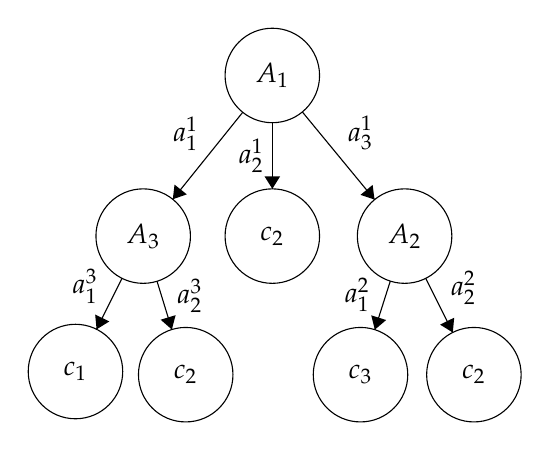
\begin{tikzpicture}[scale=0.2]
\tikzstyle{every node}+=[inner sep=0pt]
\draw [black] (18.1,-4.4) circle (3);
\draw (18.1,-4.4) node {$A_1$};
\draw [black] (9.9,-14.6) circle (3);
\draw (9.9,-14.6) node {$A_3$};
\draw [black] (5.6,-23.2) circle (3);
\draw (5.6,-23.2) node {$c_1$};
\draw [black] (12.6,-23.4) circle (3);
\draw (12.6,-23.4) node {$c_2$};
\draw [black] (18.1,-14.6) circle (3);
\draw (18.1,-14.6) node {$c_2$};
\draw [black] (26.5,-14.6) circle (3);
\draw (26.5,-14.6) node {$A_2$};
\draw [black] (23.7,-23.4) circle (3);
\draw (23.7,-23.4) node {$c_3$};
\draw [black] (30.9,-23.4) circle (3);
\draw (30.9,-23.4) node {$c_2$};
\draw [black] (16.22,-6.74) -- (11.78,-12.26);
\fill [black] (11.78,-12.26) -- (12.67,-11.95) -- (11.89,-11.33);
\draw (13.44,-8.08) node [left] {$a_1^1$};
\draw [black] (18.1,-7.4) -- (18.1,-11.6);
\fill [black] (18.1,-11.6) -- (18.6,-10.8) -- (17.6,-10.8);
\draw (17.6,-9.5) node [left] {$a_2^1$};
\draw [black] (20.01,-6.72) -- (24.59,-12.28);
\fill [black] (24.59,-12.28) -- (24.47,-11.35) -- (23.7,-11.98);
\draw (22.86,-8.07) node [right] {$a_3^1$};
\draw [black] (8.56,-17.28) -- (6.94,-20.52);
\fill [black] (6.94,-20.52) -- (7.75,-20.02) -- (6.85,-19.58);
\draw (7.05,-17.79) node [left] {$a_1^3$};
\draw [black] (10.78,-17.47) -- (11.72,-20.53);
\fill [black] (11.72,-20.53) -- (11.96,-19.62) -- (11.01,-19.91);
\draw (12.02,-18.37) node [right] {$a_2^3$};
\draw [black] (25.59,-17.46) -- (24.61,-20.54);
\fill [black] (24.61,-20.54) -- (25.33,-19.93) -- (24.38,-19.63);
\draw (24.33,-18.34) node [left] {$a_1^2$};
\draw [black] (27.84,-17.28) -- (29.56,-20.72);
\fill [black] (29.56,-20.72) -- (29.65,-19.78) -- (28.75,-20.22);
\draw (29.4,-17.89) node [right] {$a_2^2$};
\end{tikzpicture}
\caption{Example Decision Tree.}\label{fig:dt}
\end{center}
\end{figure}
\begin{figure}
\begin{lstlisting}

def DTree(D, att, class, d):
    if(d = 0):
        return Leaf(prediction=get_most_common_class(D, class))
    else:
        E_now    = Entropy(D[k+1])
        best_att = arg_max(att, lambda a: c_entropy(D, class, a))
        C = map(best_att, lambda a: DTree(D[best_att == a],
            att[att != best_att], class, d-1))
        return Node(att=best_att, children=C)
\end{lstlisting}
\caption{C4.5 Algorithm.}\label{alg:c45}
\end{figure}
When converting this mechanism to the differentially-private version, the user is left with several questions as noted in \cite{Fletcher:2016}:
\begin{itemize}
\item How large of a budget has been alotted or should be alotted? There isn't a clear way to decide the budget, as the performance of the algorithm may vary wildly with the budget.
\item How many times should the data be queried? How would pick $d$ in C4.5? Should one alter line (1) to something different?
\item Might the sensitivity of some of the queries prevent an accurate choice? Specifically, even though it is widely agreed that the entropy function performs best in the non-private setting, could a lower-quality function be substituted because its computation is more accurate?
\item How does the size of $D$ impact performance? Is there enough data to provide accurate results in the private setting?
\end{itemize}
As we will see, the answers to these questions are data-dependent and there is never one answer that always dominates.

\section{Decision Tree Examples}
For recursive decision tree algorithms set up like \ref{alg:c45}, the recursive calls on the same depth of the tree all operate on disjoint subsets of $D$. Therefore, a conservative estimate of the privacy usage, using composition and disjointness, is
\begin{equation}
\sum_{i=0}^d \max_{n \in \texttt{Nodes on lvl }i} \epsilon_{n}
\end{equation}
where $\epsilon_n$ is the privacy used by node $n$. We will go into details on how to pick $\epsilon_n$ later
The most naive way to create a DP version of C4.5 is to take all the histogram queries in algorithm \ref{alg:c45} and change them to \texttt{NoisyCount}. This results in the following code for \texttt{c\_entropy}
\begin{lstlisting}
def c_entropy(D, class, attribute):
    N = NoisyCount(D)
    for a in attribute:
        count_a = NoisyCount(D[attribute == a])
\end{lstlisting}
\begin{theorem}
The entropy function on disjoint histogram counts $a_1,a_2,\ldots, a_n$ produced from a database $D$ has sensitivity bounded by $\frac{1}{|D|}\left(\frac{1}{\ln(2)} + \log(|D|) \right)$.
\end{theorem}
\begin{proof}
Let $A = \sum_{i=1}^n a_i$. Then, the entropy is 
\[
\sum_{i=1}^n \frac{a_i}{A}\log\left(\frac{A}{a_i}\right) = \frac{1}{A}\sum_{i=1}^n a_i\log A - \frac{1}{A} \sum_{i=1}^n a_i\log(a_i) = \log(A) - \frac{1}{A}\sum_{i=1}^n a_i\log(a_i)
\]
Suppose bucket $a_j$ is reduced by 1, and the entropy change is
\begin{align*}
&\log(A) - \log(A-1) - \frac{1}{A} a_j\log(a_j) + \frac{1}{A-1} (a_j-1)\log(a_j-1) \\
&\leq \frac{1}{\ln(2)(A-1)} -\frac{1}{A}(a_j-1)\log(a_j-1) + \frac{1}{A-1}(a_j-1)\log(a_j-1) \\
&= \frac{1}{\ln(2)(A-1)}+\frac{1}{A(A-1)}(a_j-1)\log(a_j-1) \leq \frac{1}{\ln(2)(A-1)} + \frac{1}{A}\log(A)
\end{align*}

\end{proof}

\bibliographystyle{plain}
\bibliography{Thesis}
\end{document}